
\section{Data and Query Model}
\label{sec:queryModel}

We first provide a short review of Datalog, following the conventions
in Ramakrishnan and Ullman's survey~\cite{ramakrishnan93survey}. A 
Datalog program consists of a set of declarative {\em rules} and a
query. A Datalog {\em rule} has the form {\em p :- 
$q_{1}, q_{2}, ..., q_{n}$}., which can be read informally as
``$q_{1}$ and $q_{2}$ and $ ... $ and $q_{n}$ implies p''. $p$ is the {\em head} of the
rule, and $q_{1}, q_{2}, ..., q_{n}$ is a list of {\em literals} that
constitutes the {\em body} of the rule.  Literals are either {\em
predicates} applied to {\em fields} (variables and constants), or
function symbols applied to fields. The rules can refer to each other
in a cyclic fashion to express recursion. The order in which the rules
are presented in a program is semantically immaterial.  The commas
separating the predicates in a rule are logical conjuncts ({\em AND});
the order in which predicates appear in a rule body also has no
semantic significance (though implementations typically employ a
left-to-right execution strategy). The query
specifies the output of interest. 

The predicates in the body and head of Datalog rules are relations,
and we will refer to them interchangeably as predicates, relations, or
tables.  Each relation has a {\em primary key}, which consists of a
set of fields that uniquely identifies each tuple within the
relation. We allow the primary key to be specified for stored
(``extensional'') relations; in the absence of other information, the
primary key is the full set of attributes in the relation. 
%RR If you decide to remove the stuff on keys, perhaps you should
%drop the underlining convention below \ldots
%In our schema
%definitions, we \underline{underline} the primary key attributes of a
%table (unless the primary key is the full set of attributes).    
%\footnote{If
%  the primary key is not the full set of attributes, there can be multiple tuples generated with the same primary
%  key. In this case, the results set contains one of the derivations,
%  depending on the evaluation strategy and execution run.}. 

The names of predicates, function symbols
and constants begin with a lower-case letter,
while variable names begin with an upper-case letter.  Most
implementations of Datalog enhance it with a limited set of function
calls (which start with {\em ``f\_''} in our syntax), including
boolean predicates, arithmetic computations and simple list
manipulation (\eg the $f\_concatPath$ function in our first
example). Aggregate constructs are represented as functions with field
variables within angle brackets ($<>$). For most of our discussion, we
will not consider negated predicates; we will return to the topic of
negation as part of our future work (Section~\ref{sec:futurework}).

As an example, the following program computes the shortest paths between
all pairs of nodes in a graph. The program has four rules (which for
convenience we label R1-R4), and takes as input a stored
(``extensional'') relation $link(src, dst, cost)$.  R1 and R2 are used
to derive ``paths'' in the graph, represented as tuples in the
derived (``intensional'') relation $path(src, dst, nextHop, pathVector, \ldots)$.  The $src$ and
$dst$ fields represent the endpoints of the path; the $pathVector$ is
a string encoding the full path. We discuss $nextHop$ later. Given the
$path$ relation, Rule R4
computes the shortest paths as the derived relation
$shortestPath(src, dst, pathVector, cost)$. R3
derives the relation $spCost(src, dst, mincost)$ that
computes the minimum cost for each (src,dst) group for all input paths.
The rule {\em Query} specifies shortestPath tuples as the result
tuples. R2 is a {\em linear} rule, since there is only one
recursive literal in the body. Rules with more than one recursive literal
in the body are {\em non-linear}.

%In this example, {\em S}, {\em Z}, {\em D}, {\em C} and {\em P}
%abbreviate the {\em source}, {\em nextHop}, {\em destination}, {\em
%cost} and {\em pathVector} fields respectively for both the link and
%path tuples.    

\vspace{2pt} {\small
\noindent{\bf R1: } path(S,D,D,P,C) :- link(S,D,C), P = $f\_concatPath$(link(S,D,C), nil). \\
{\bf R2: } path(S,D,Z,P,C) :-
  link(S,Z,C$_{1}$), path(Z,D,Z$_{2}$,P$_{2}$,C$_{2}$),\\
\datalogspace C = C$_{1}$ + C$_{2}$, P = $f\_concatPath$(link(S,Z,C$_{1}$),P$_{2}$).\\
{\bf R3: } spCost(S,D,min$<$C$>$) :- path(S,D,Z,P,C).\\
{\bf R4: } shortestPath(S,D,P,C) :- spCost(S,D,C), path(S,D,Z,P,C).\\
{\bf Query: } shortestPath(S,D,P,C).
}
\vspace{2pt}

Rule R1 produces one-hop paths from existing link tuples, and Rule R2
recursively produces path tuples of increasing cost by matching the
destination fields of existing links to the source fields of previously
computed paths. The matching is expressed using the repeated ``Z'' variable in
$link(S,Z,C_{1})$ and $path(Z,D,Z_{2},P_{2},C_{2})$ of rule
R2. Intuitively, rule R2 says that if there is a link from node {\em S}
to node {\em Z}, and there is a path from node {\em Z} to node {\em D},
then there is a path from node {\em S} to node {\em D} via {\em Z}. In
the presence of path cycles, the query never 
terminates, as R1 and R2 will generate paths of ever increasing
lengths. However, this can be fixed with a well-known query rewrite 
(Section~\ref{subsec:aggregateSelections}) when costs are positive.% $\gt$ 0.  

%The query does not impose any restriction on either source or
%destination as both {\em S} and {\em D} are unbound
%variables. Hence, the query computes the {\em full transitive
%closure} consisting of the paths between all pairs of reachable
%nodes. If the query is only interested in the paths from a given
%node {\em b} to every other node in the network, the query would be
%$path({\bf b},D,P,C)$, with the source field bound to
%constant {\em b}.

%R3 and
%R4 together are then used to compute the shortest paths from the
%computed paths. 

\subsection{Network Datalog}

In this section, we introduce the data and query model that we propose
for declarative networking. The language we present is {\em Network
  Datalog} (\Dlog), a restricted variant of traditional Datalog intended
to be computed in distributed fashion on physical network graphs.  In
describing our model, we use the \Dlog query shown in
Figure~\ref{shortestPath}, which performs distributed computation of
shortest paths.


\begin{figure}[ht]
\begin{boxedminipage}{3.2in}
{\small
\noindent{\bf SP1: } path({\bf @S},@D,@D,P,C) :- \link({\bf @S},@D,C), \\
\datalogspace P = $f\_concatPath$(link({\bf @S},@D,C), nil). \\
{\bf SP2: } path({\bf @S},@D,@Z,P,C) :-
  \link({\bf @S},@Z,C$_{1}$), \\
\datalogspace path({\bf @Z},@D,@Z$_{2}$,P$_{2}$,C$_{2}$), C = C$_{1}$ +
C$_{2}$, \\
\datalogspace P = $f\_concatPath$(link({\bf @S},@Z,C$_{1}$),P$_{2}$).\\ 
{\bf SP3: } spCost({\bf @S},@D,min$<$C$>$) :- path({\bf @S},@D,@Z,P,C).\\
{\bf SP4: } shortestPath({\bf @S},@D,P,C) :-
spCost({\bf @S},@D,C),\\
\datalogspace path({\bf @S},@D,@Z,P,C).\\
{\bf Query: } shortestPath({\bf @S},@D,P,C).
}
\end{boxedminipage}
\small{\caption{\label{shortestPath}\emph{\small Shortest-Path
      Query in \Dlog}.}}
\end{figure}

One of the novelties of our setting, from a database perspective, is
that data is distributed and relations may be partitioned across
sites.  To ease the generation of efficient query plans in such a
system, \Dlog gives the query writer {\em explicit} control on data
placement and movement. Specifically, \Dlog uses a special data type,
{\em address}, to specify a network location.  Names of address
variables and constants are prepended with ``@''.  More formally, we
have the following definition:

\begin{Def}{\em A {\em location specifier} is an attribute of type
    address in a predicate that indicates the network storage
    location of each tuple.}
\end{Def}

As a matter of notation, we require the location specifier to be the
first field in all predicates, and we highlight it in {\bf bold} for
clarity. For example, the location specifier of $link$({\bf @S},@D,C) is {\bf @S}.

Another novelty of our setting is that we assume a network graph that
is not fully connected, \ie a node can communicate {\em directly}
with only a subset of nodes in the system.  This allows us to model
the physical connectivity of a typical autonomous system in the
Internet, where each node is connected to relatively few other nodes.
In contrast, both traditional parallel query processors and more
recent distributed query engines, such as PIER~\cite{pierCidr}, assume a
fully connected network graph, where messages can be sent directly
from any node to any other node in the system.  Parallel systems
achieve this by engineering (and provisioning) the interconnection
network, while PIER uses overlay routing to connect any two nodes.

%Our network setting is different, since the goal of networking is to
%{\em provide} full end-to-end connectivity rather than assuming it
%ahead of time. Consequently, we assume physical connectivity is
%incomplete (the normal case in a link-based network), and impose the
%constraint that messages (e.g., tuples participating in distributed
%joins) can only be exchanged between two nodes that are connected by a
%link.

To express the constraint that a node can send data only to another node with which it is
physically connected, we introduce the concept of {\em link relation},
which is defined as follows:

%Again, we want to expose this in the query language to facilitate the
%specification of messaging in the network graph.  Hence we introduce
%the following notion:

\begin{Def}{\em A {\em link relation} is a stored (``extensional'')
     relation \\$link(@src, @dst, ...)$ representing the connectivity
     information of the network being queried.}\end{Def}

%Links are defined
%using the following DDL: \texttt{linktbl
%  <tblname>(@S,@D [,<othercols>])}. 
The first two fields of each link table entry contain the source and
destination addresses of a network link respectively, followed by an
arbitrary number of other fields (typically metrics) describing the
link.  In this paper, we constrain all links to be
bidirectional, \ie if there is
a network edge from a node to its neighbor, the reverse must be true\footnote{In practice, some networks may not have
symmetric links.  Our framework can be extended to handle this, but
generalizing the discussion in that manner complicates our
presentation and is out of the scope of this paper.}.
In all our example queries, we utilize only one link table. In
practice, there can be multiple such tables used by different rules.
% , but to simplify our
% exposition we focus on a single link table in this paper.  We denote link relations
% with the syntax \link.  

Given that we will be executing queries across network links, it is useful to identify queries that do not require communication:
\begin{Def}{\em {\em Local rules} are rules that have the same
	location specifier in each predicate, including the
	head.}\end{Def}

%\begin{Def}{\em {\em Local body rules} are rules that have the same
%	location specifier in each body predicates. }\end{Def}

Local rules can be executed without any distributed logic.  Rules SP1,
  SP3 and SP4 are local. SP2 is a non-local rule since the
  $link$ and $path$ body predicates are stored at different
  locations. 

In \Dlog, the evaluation of a rule must depend only on communication
along the physical links. To this end, we introduce the following:
\begin{Def}{\em A {\em link literal} is a link relation that appears
in the body of a rule prepended with the ``\#'' symbol.}
\end{Def}
Given the preceding definitions, we are ready to define a simple
syntactic constraint on the rules to ensure that communication takes
place only along the physical links:

\begin{Def}\label{def:topRestricted} {\em A {\em link-restricted} rule
    is either a local rule, or a rule with the following properties:
\begin{mylist}
\item There is exactly one link literal in the body
\item All other literals (including the
      head predicate) have their
  location specifier set to either the first (source) or second
  (destination) field of the link literal. 
\end{mylist}}
\end{Def}

This syntactic constraint precisely captures the requirement that we
be able to operate
directly on a network whose link connectivity is not a full mesh.
Further, as we demonstrate in Section~\ref{sec:queryPro}, link-restriction
also guarantees that all programs with only link-restricted
rules can be rewritten into a canonical form where every rule body can be
evaluated on a single node. In addition, all communication for each
rewritten rule only involves sending messages along links. The
following is an example of a link-restricted rule:\\
\vspace{2pt}
{\small 
\noindent p({\bf @D},...) :- \link({\bf @S},@D,...),p$_{1}$({\bf
  @S},...),p$_{2}$({\bf @S},...), ..., p$_{n}$({\bf @S},...).
}
\vspace{2pt}

The rule body of this example is executed at @S and the resulting $p$
tuples are sent to @D, preserving the communication constraints along
links. Note that this example's body predicates all have the same
location specifier: @S, the source of the link. In contrast, rule SP2
of Figure~\ref{shortestPath} is link-restricted but has some relations whose location
specifier is the source, and others whose location specifier is the
destination; this needs to be rewritten as described in Section~\ref{sec:queryPro}. 
%A query rewrite technique described in
%Section~\ref{sec:queryPro} transforms such rules to ensure all body
%predicates are at the same location; we will apply this rewrite to all
%eligible rules to simplify our execution.


%In practice, there can be multiple topology tables used
%concurrently within a single message rule. One example is in specifying
%the Chord DHT~\cite{chord}, which requires three topology tables
%($finger$, $successor$ and $predecessor$) that can be used concurrently
%within a single rule. We do not address the use of multiple topology
%tables within a single rule in this paper.

Given these preliminaries, we are now ready to present our language \Dlog:

\begin{Def}{\em A Network Datalog (\Dlog) program is a Datalog program that satisfies
    the following syntactic constraints:
\begin{myenumerate}
\item {\bf Location specificity:} Each predicate has a location
  specifier as its first attribute 
\item {\bf Address type safety:} A variable that appears once in a
  rule as an address type must not appear elsewhere in the rule
  as a non-address type.
\item {\bf Stored link relations:} Link relations never appear in the head of a rule with a
  non-empty body (\ie they are stored, not derived).
\item {\bf Link-restriction:} Any non-local rules in the program are
  link-restricted by some link relation.
\end{myenumerate}
}
\end{Def}
Since \Dlog is a subset of Datalog, the semantics of a valid \Dlog
program are exactly those of Datalog.

\subsection{Shortest Path Example}
\label{sec:queryExec}
To illustrate \Dlog, we step through an execution of the {\em
shortest-path} query above to illustrate derivation and communication
of tuples as the query is computed. We make use of the example network
in Figure~\ref{SP example}.  Our discussion is necessarily informal
since we have not yet presented our distributed implementation
strategies; in the next section, we show in greater detail the steps
required to generate the execution plan.  Here, we focus on a
high-level understanding of the data movement in the network during
query processing.

%Here,
%  we also assume that there are no updates to the network during query
%  execution, and relax this assumption in later sections.

\begin{figure}[ht]
\centering
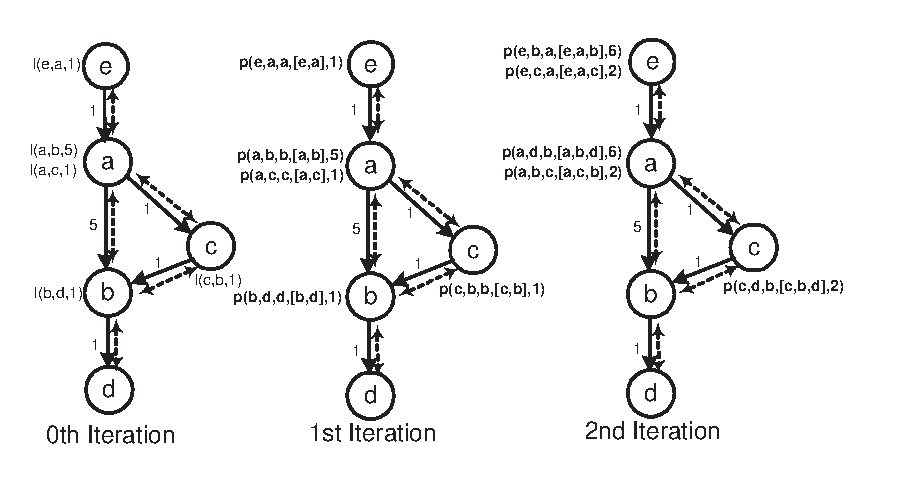
\epsfig{file=images/example.eps, width=3.5in}
\caption{\label{SP example}\emph{\small Nodes in the
    network are running the shortest-path query. We only show newly
    derived tuples at each iteration. For
    simplicity, we show only the derived paths along the
    solid lines even though the network connectivity is bidirectional (dashed lines).}}
\end{figure}                                              

We will describe communication in {\em iterations}, where at each
iteration, each network node generates $paths$ of increasing hop count, and then
propagates these paths to neighbor nodes along links. In the $1^{st}$
iteration, all nodes initialize their local path tables to 1-hop
paths using SP1. In the $2^{nd}$ iteration, using SP2, each node takes the input
paths generated in the previous iteration, and computes 2-hop paths,
which are then propagated to its neighbors. For example, $path({\bf
  a},d,b,[a,b,d],6)$ is generated at node {\em b} using
$path(b,d,d,$ $[b,d],1)$ from the $1^{st}$ iteration, and propagated to node
{\em a}. In addition to storing the entire path vector, each $path$
tuple also contains the {\em nextHop} attribute, which indicates for each path the next hop to
route the message in the network. In fact, many network protocols
propagate only the {\em nextHop} and avoid sending the entire path vector.

As paths are being computed, the shortest paths are also
incrementally computed. For example, node $a$ computes $path({\bf
  a},b,b,[a,b],5)$ using rule SP1, and then sets its shortest path to
$shortestPath({\bf a},b,$ $[a,b],5)$ using rule SP4. In the next iteration, node $a$
receives $path({\bf a},b,c,$ $[a,c,b],2)$ from node $c$ which has lower cost
compared to the previous shortest cost of 5, and hence a new $shortestPath({\bf a},b,[a,b],2)$ replaces the previous value.

%In the distributed implementation, the use of an optimization (described in Section~\ref{subsec:aggregateSelections})
%requires each node to only propagate its current shortest path to its
%neighbor node. In that case, each node only needs to maintain the
%current shortest path to every destination reported by each
%neighbor. 
%In this case, the primary key for $paths$ is
%(src,dst,nextHop).  



%This iteration is akin to
%that used in {\em semi-\naive}~\cite{semi, semi1} fixpoint evaluation techniques in traditional Datalog
%evaluation. In practice, query execution is fully asynchronous, tuples for the next round can be generated as soon as
%tuples from the previous round are computed. We will revisit this model
%of execution in later sections.




\subsection{Expressiveness}
\label{subsec:shortestPath}

In previous work~\cite{declareRoute} we argued that executing a shortest path
distributed 
Datalog query closely resembles the distributed computation of the well-known
path vector~\cite{ee122text} protocol.  In proposals for
declarative networks~\cite{declareRoute,declareOverlays}, Datalog-like programs were used
for a variety of networking tasks, including
standard routing protocols such as {\em distance
  vector}~\cite{ee122text} and {\em dynamic source
  routing}~\cite{dsr}, and more complex networks such as multicast trees
and the Chord network~\cite{chord}.  We note that \Dlog is
flexible enough for expressing most of these programs efficiently, and provides the advantages of having clear
semantics as described above (something that is not available in the
original language for \Sys described in~\cite{declareOverlays}) and a clearly defined
link-restricted implementation as described below.

%The {\em shortest-path} query is a variant of
%transitive closure computation. With minor variations, we can specify well-known
%routing protocols performing transitive closure computations. These
%include {\em distance vector}~\cite{ee122text}, {\em
%  dynamic source routing}~\cite{dsr}, best-k paths, paths with quality
%of service constraints, etc.

%Instead of computing the shortest path, by modifying
%the ``+'' and ``min'' aggregate, we can compute other types of shortest
%paths, such as the most reliable or the three least bottleneck
%paths. 
%We provide an example below that allows one to incorporate {\em
%  policy} restrictions easily on the computed shortest paths:

%\vspace{2pt}
%{\small
%\noindent{{\bf \#include(SP1,SP3,SP4)}} \\
%{\bf PR2: } path({\bf @S},@Z,@D,P,C) :-
%  \link({\bf @S},@Z,C$_{1}$), \\
%\datalogspace path({\bf @Z},@Z,$_{2}$,@D,P$_{2}$,C$_{2}$),\\
%\datalogspace excludeNode({\bf @Z},@W), C = C$_{1}$ + C$_{2}$, \\
%\datalogspace P =
%$f\_concatPath$(\link({\bf @S},@Z,C$_{1}$),P$_{2}$).\\
%{\bf Query: } shortestPath({\bf @S},@D,P,C).
%}
%\vspace{2pt}

%In this query, we introduce an additional table {\em excludeNode},
%where $excludeNode({\bf S},W)$ is a tuple that
%represents the fact that node {\em S} does not carry any traffic for
%node {\em W}. This $excludeNode$ is considered an optional predicate and
%is stored at the same location as $path$.

%To show that the restrictions do not constrain us to solely transitive closure
%computations, we present the following program below that implements the
%link flooding component of the {\em link-state}~\cite{ee122text} protocol: 

%\vspace{2pt}
%{\small
%\noindent{{\bf LS1: } flood\link({\bf @D},@S,@S,@D,C) :-
%  \link({\bf @S},@D,C)} \\
%{\bf LS2: } flood\link({\bf @M},@N,@S,@D,C) :- \link({\bf @N},@M,C$_{1}$),\\
%\datalogspace flood\link({\bf @N},@W,@S,@D,C), @M $\ne$ @W. \\
%{\bf Query: } flood\link({\bf @M},@N,@S,@D,C)
%}
%\vspace{2pt}

%flood\link({\bf @M},@N,S,D,C) is a message predicate, and
%each is tuple storing information
%about {\em \link(S,D,C)}. This tuple is flooded in the network starting
%from source node {\em S}. During the flooding process, node @M is the
%current node it is flooded to, while node @N is the node that forwarded
%this tuple to node {\em M}.  Rule LS1 generates a $floodlink$ tuple for every
%link at each node. Rule LS2 states that each node {\em N} that receives
%a $floodlink$ tuple recursively forwards the tuple to all neighbors {\em M}
%except the node {\em W} that it received the tuple from


%\subsection{Incremental Negation Evaluation}
%Negation has to stratified and computed locally. 



%\subsection{Query Convergence}

%In a static network, the query for computing all-pairs shortest paths converges in the same time
%as the diameter (in hops) of the network. However, the presence of cycles can lead
%to infinite messages. This is preventable if there is a mechanism of
%``bounding'' the recursion. Typically, this is done by not permitting
%path cycles, or enforcing bounds on the cost arguments of messages. For the latter, we have
%to enforce that all functions used in link
%structure recursion to derived tuples have cost arguments that are 
%monotonically increasing/decreasing, and queries are on bounds of these
%cost arguments or min/max aggregates. Aggregates provide a bound with
%the use of aggregate selections
%optimizations in Section~\ref{sec:queryOpt}. 


%One thing to note is that while the final query
%results for shortestPath is the same for the same input network, the intermediate paths
%generated may differ based on network dynamics and reordering of
%messages (affects how pruning is done). For example, if node a receives
%$path(a,b,c,[a,c,b],2)$ before $path(a,b,b,[a,b],5)$, then
%$path(e,b,a,[e,a,b],6)$ would not be generated due to aggregate
%selections. However, in either case, this does not affect the final
%$shortestPath(e,b,[e,c,b],2)$ being computed.




%We are not restricted to generalized transitive closure
%computations. For example, link state:%

%\vspace{2pt}
%{\small
%\noindent{{\bf LS1: } flood\link(@S},@S,@D,C,@S) :- \link(@S},@D,C)} \\
%{\bf LS2: } flood\link(@M},@S,@D,C,@N) :- \link(@N},@M,C$_{1}$),\\
%\datalogspace flood\link(@N},@S,@D,C,@W), M $\ne$ W. \\
%{\bf Query: } flood\link(@M},@S,@D,C,@N)
%}
%\vspace{2pt}


